%Admin
\textbf{Autor: Arbnor, Torben} \\
In diesem Kapitel beschreiben wir Anleitungen zur Nutzung der Grade+ Anwendung für Nutzer mit der Rolle Admin. Dabei gehen wir detailliert auf alle relevanten Punkte für die Rolle des Admins ein.\\
In Abbildung \ref{fig 1} ist das Menü / der Header eines Nutzers mit der Rolle Admin zu sehen. 
Im folgenden werden die Menüpunkte Nutzerverwaltung (Kapitel  \ref{nutzerverwaltung}), Datensicherung(Kapitel  \ref{datensicherung}) und User-Profil (Kapitel  \ref{profil}) weiter erläutert.
\begin{figure}[H]
	\centering
	\caption{Header/Menü-Leiste des Admin}
  
\includegraphics[width=\textwidth,height=10cm,keepaspectratio]{../screenshots/Admin/menu.png}
	\label{fig 1}
\end{figure}

%%%%%%%%%%%%%%%%%%%%%%%%
\subsection{Nutzerverwaltung}
\label{nutzerverwaltung}
Unter der Nutzerverwaltung sind die Funktionen zur Registrierung von Prüfer und Admin untergebracht. 
\subsubsection{Registrierung von Prüfer und Admins}  \label{sec:regPuA}

\begin{figure}[H]
	\centering
	\caption{Header/Menü-Leiste des Admin}
  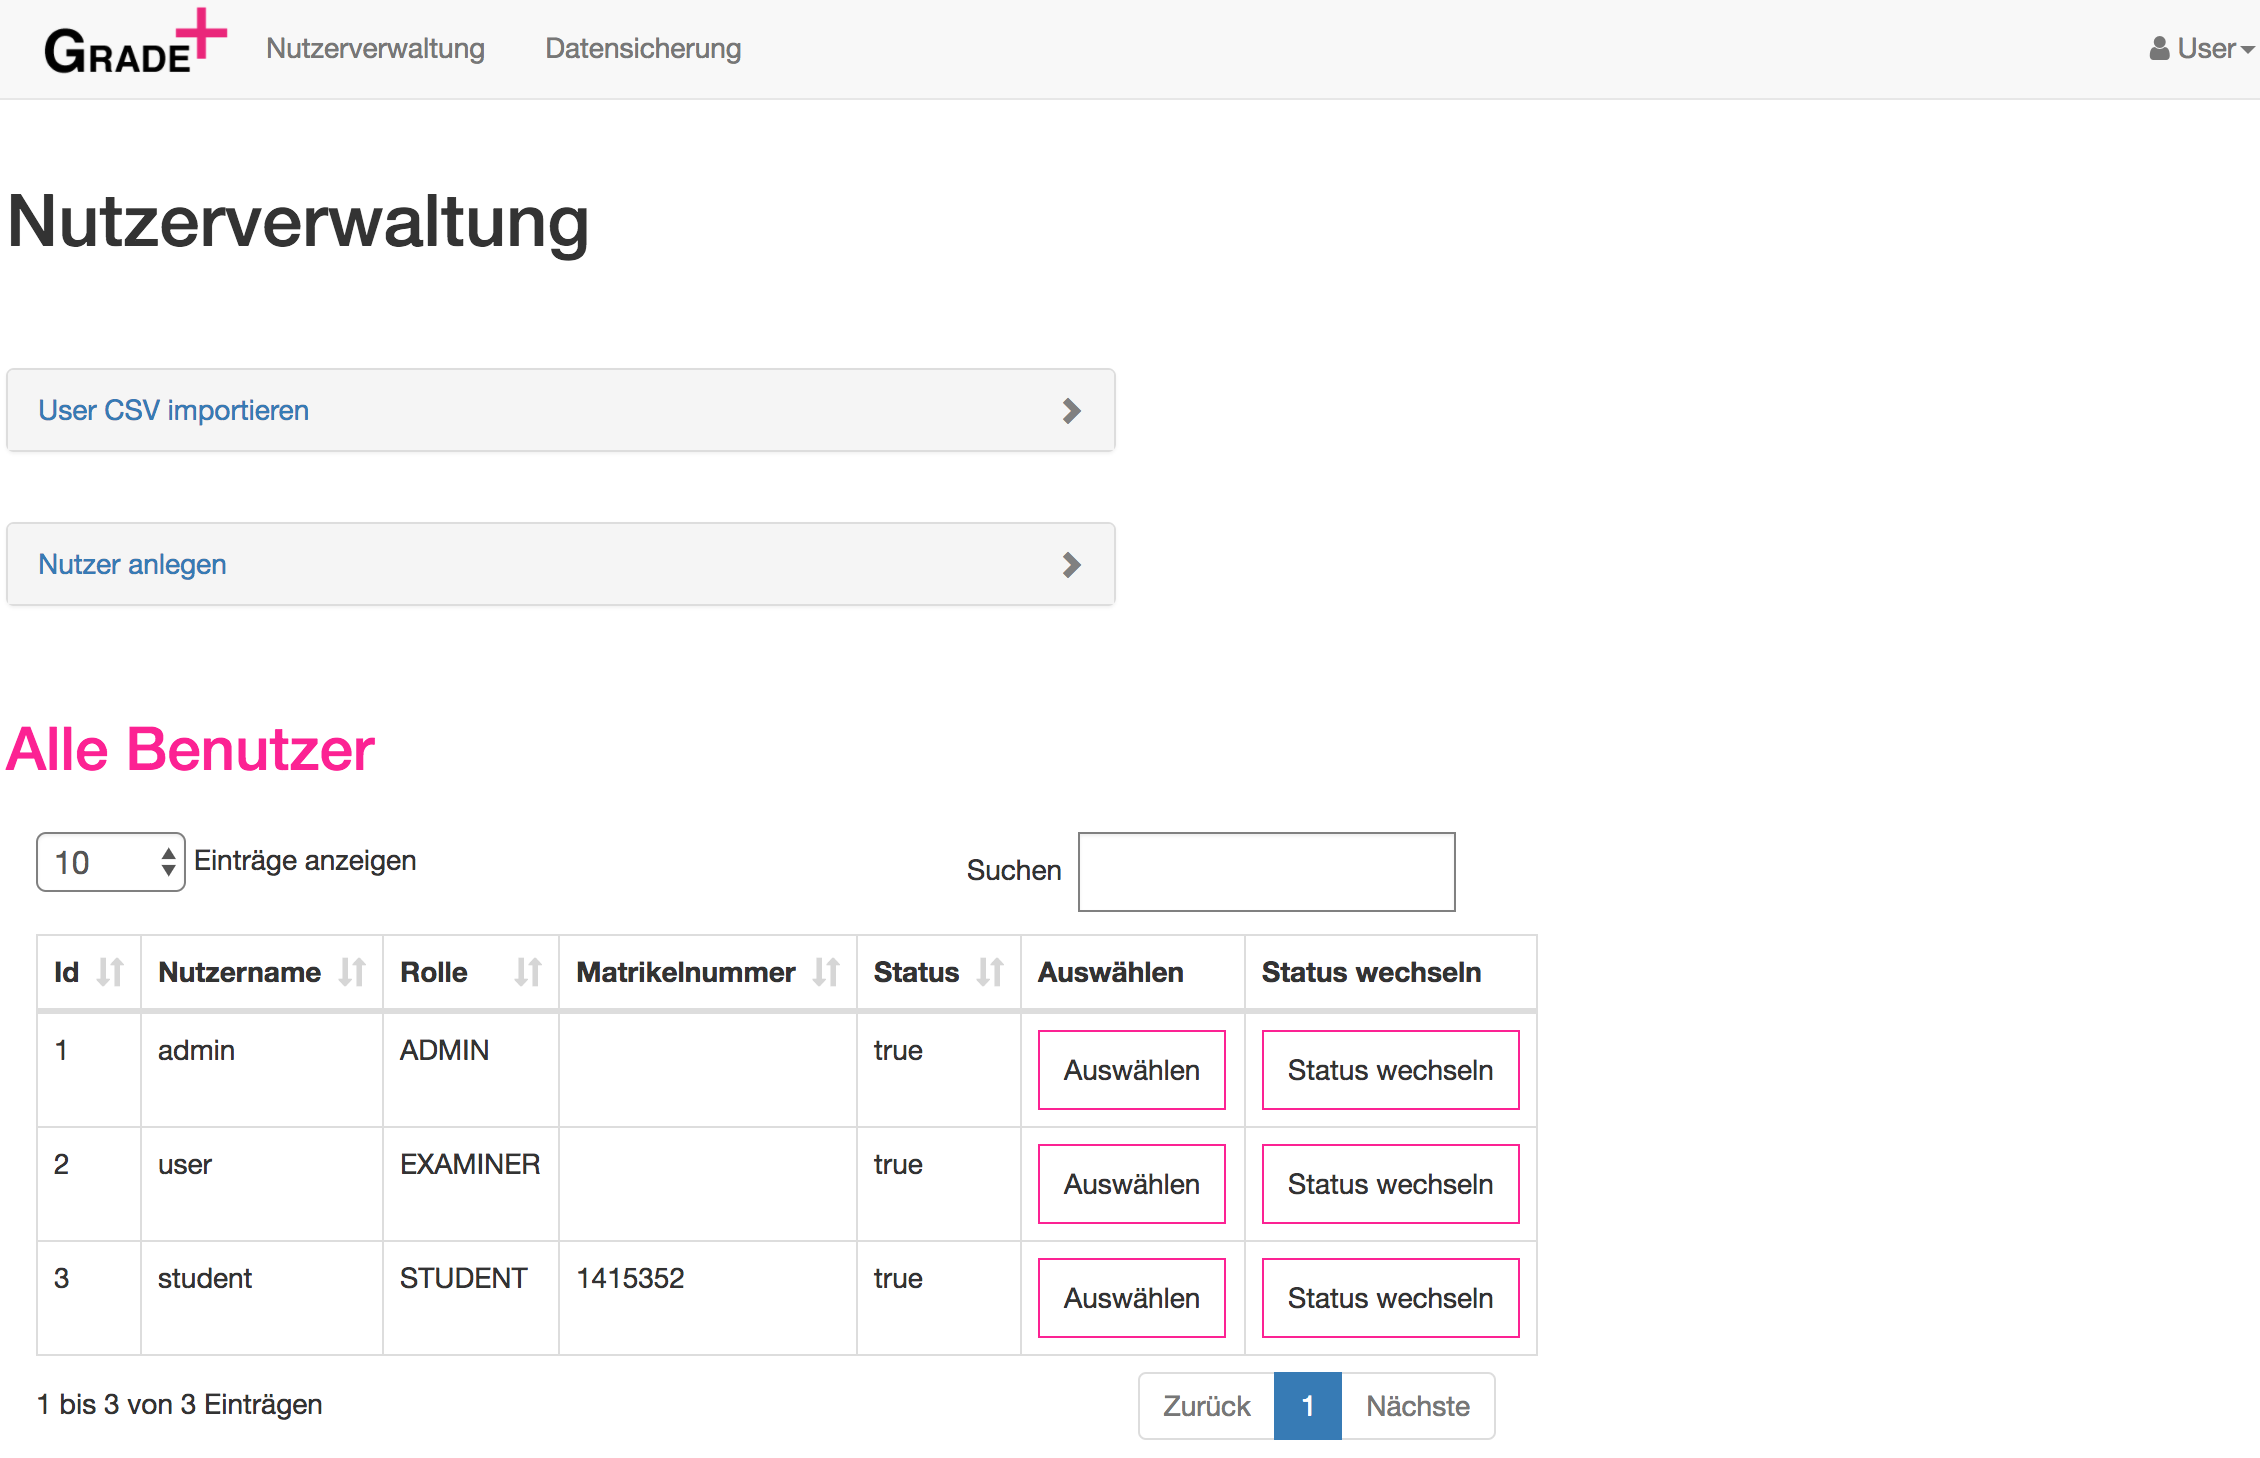
\includegraphics[width=\textwidth,height=10cm,keepaspectratio]{../screenshots/Admin/Nutzerverwaltung/nutzer1.png}
	\label{fig 2}
\end{figure}


%%%%%%%%%%%%%%%%%%%%%%%%

\subsection{Datensicherung}
\label{datensicherung}

\subsubsection{Backup erstellen}
\subsubsection{Backup einspielen}
\subsubsection{Backup löschen}

%%%%%%%%%%%%%%%%%%%%%%%%
\subsection{Profil  bearbeiten}
\label{profil}
%%%%%%%%%%%%%%%%%%%%%%%%


